% 1. Summary Statistics
\input{Tables_Figures/SummaryStats}
\clearpage
% 2. Balance Table
\input{Tables_Figures/BalanceTest}
\clearpage
% 3. Transfer In
\input{Tables_Figures/NewTable1_Reallocation}
\clearpage
% 4. Transfer Decomposition by Distance
\input{Tables_Figures/NewTable1c_TransferType}
\clearpage
% 5. Retention
\input{Tables_Figures/NewTable3_Retention}
\clearpage
% 5. Salary Increase (Rinji Tokubetsu)
\input{Tables_Figures/NewTable4_Rinji}
\clearpage
% 6. Promotion (Short-Run)
\input{Tables_Figures/NewTable5_Promotion}
\clearpage
% 7. New Hires at Impacted Office
\input{Tables_Figures/NewTable1b_NewHires}
\clearpage
% 8. Gender Composition
\input{Tables_Figures/NewTable2_Gender}
\clearpage
% 9. Future Outcomes (Long-Run)
\input{Tables_Figures/NewTable3_FutureOutcomes}
\clearpage
% 10. Headcount Regression: Effect of Drafting on Office Size
\input{Tables_Figures/HeadcountRegression}
\clearpage
% 11. Donor Office Descriptive Stats (Contemporaneous)
\begin{table}[htbp]
\centering
\caption{Characteristics of Donor Offices (Offices with Transfers Out)}
\label{tab:donor}
\small
\begin{threeparttable}

\textbf{Panel A: Unconditional Comparison}
\medskip

\begin{tabular}{lcccccc}
\toprule
 & \multicolumn{2}{c}{Donor} & \multicolumn{2}{c}{Non-Donor} & & \\
 & Mean & SD & Mean & SD & Diff & $p$-value \\
\midrule
Has New Hire (=1) & 0.729 & 0.445 & 0.552 & 0.497 & 0.177 & $<$0.001 \\
No. New Hires & 9.251 & 18.899 & 3.317 & 9.719 & 5.934 & $<$0.001 \\
Avg Tenure (years) & 2.880 & 1.301 & 2.636 & 1.516 & 0.245 & $<$0.001 \\
Female Share & 0.026 & 0.079 & 0.044 & 0.142 & -0.019 & $<$0.001 \\
\bottomrule
\end{tabular}

\bigskip

\textbf{Panel B: Conditional Comparison (Kyoku + Position + Year FE)}
\medskip

\begin{tabular}{lccccc}
\toprule
 & Coef & SE & $t$-stat & $p$-value & $N$ \\
\midrule
Has New Hire (=1) & 0.0774$^{**}$ & 0.0343 & 2.26 & 0.024 & 6,603 \\
No. New Hires & 3.9355$^{**}$ & 1.7100 & 2.30 & 0.022 & 6,603 \\
Avg Tenure (years) & 0.1218$^{***}$ & 0.0364 & 3.34 & $<$0.001 & 6,603 \\
Female Share & -0.0079$^{**}$ & 0.0035 & -2.29 & 0.022 & 6,603 \\
\bottomrule
\end{tabular}

\begin{tablenotes}[flushleft]
\footnotesize
\item \textit{Notes:} Sample: ka $\times$ position $\times$ year (1938--1945). A \emph{donor} office is one that had at least one worker transfer out in that year. Panel~A reports unconditional means. Panel~B reports coefficients from OLS regressions of each characteristic on a donor indicator, with kyoku, position, and year fixed effects, controlling for log office headcount. Standard errors clustered at the office level. $^{***}p<0.01$, $^{**}p<0.05$, $^{*}p<0.1$.
\end{tablenotes}
\end{threeparttable}
\end{table}

\clearpage
% 11b. Donor Office Lagged Hiring Test (Vacancy Chains vs Selection)
\begin{table}[htbp]
\centering
\caption{Lagged Hiring Test: Prior-Year Outcomes by Future Donor Status}
\label{tab:donor_lagged}
\small
\begin{threeparttable}

\textbf{Panel A: Unconditional Comparison}
\medskip

\begin{tabular}{lcccccc}
\toprule
 & \multicolumn{2}{c}{Future Donor} & \multicolumn{2}{c}{Non-Donor} & & \\
 & Mean & SD & Mean & SD & Diff & $p$-value \\
\midrule
Has New Hire (=1) & 0.696 & 0.460 & 0.478 & 0.500 & 0.218 & $<$0.001 \\
No. New Hires & 7.447 & 17.243 & 1.867 & 4.813 & 5.580 & $<$0.001 \\
Avg Tenure (years) & 2.724 & 1.294 & 3.237 & 1.908 & -0.513 & $<$0.001 \\
Female Share & 0.034 & 0.098 & 0.046 & 0.158 & -0.012 & $<$0.001 \\
\bottomrule
\end{tabular}

\bigskip

\textbf{Panel B: Conditional Comparison (Kyoku + Position + Year FE + Log Headcount at $t$)}
\medskip

\begin{tabular}{lccccc}
\toprule
 & Coef & SE & $t$-stat & $p$-value & $N$ \\
\midrule
Has New Hire (=1) & 0.1603$^{***}$ & 0.0156 & 10.29 & $<$0.001 & 7,235 \\
No. New Hires & 5.1419$^{***}$ & 0.6665 & 7.71 & $<$0.001 & 7,235 \\
Avg Tenure (years) & 0.1133$^{***}$ & 0.0289 & 3.92 & $<$0.001 & 7,235 \\
Female Share & -0.0081$^{**}$ & 0.0032 & -2.53 & 0.012 & 7,235 \\
\bottomrule
\end{tabular}

\begin{tablenotes}[flushleft]
\footnotesize
\item \textit{Notes:} This table tests whether the new-hiring gap between donor and non-donor offices reflects vacancy chains or selection. Outcomes (new hires, tenure, female share) are measured at year $t{-}1$; donor status is defined at year $t$ (whether the office had any transfers out). If offices that will become donors already exhibit higher hiring rates in the prior year, this suggests selection rather than vacancy chains. Sample: ka $\times$ position, outcome years 1937--1944, donor status years 1938--1945. Panel~A reports unconditional means. Panel~B reports coefficients from OLS regressions with kyoku, position, and year fixed effects, controlling for log office headcount at year $t$. Standard errors clustered at the office level. $^{***}p<0.01$, $^{**}p<0.05$, $^{*}p<0.1$.
\end{tablenotes}
\end{threeparttable}
\end{table}

\clearpage
% 12. Characteristics of Transferred Workers
\input{Tables_Figures/TransferredWorkerChars}
\clearpage
% 13. Postwar Outcomes for Donor Offices
\input{Tables_Figures/DonorPostwarOutcomes}
\clearpage
% 14. Network Proximity and Transfer Selection
\input{Tables_Figures/NetworkProximity}
\clearpage
% 15. Long-Run Outcomes of Transferred Workers
\begin{table}[htbp]
\centering
\caption{Long-Run Outcomes of Transferred Workers}
\label{tab:transfer-outcomes}
\begin{threeparttable}

\textbf{Panel A: Transferred vs.\ Destination Office Peers}
\medskip

\begin{tabular}{lcccc}
   \tabularnewline \midrule \midrule
                        & Tenure After   & Postwar Surv.      & Postwar Yrs     & Rank Gain \\   
   Model:               & (1)            & (2)                & (3)             & (4)\\  
   \midrule
   \emph{Variables}\\
   Transferred (=1)     & 0.6888$^{***}$ & 0.0436$^{***}$     & 0.1325$^{***}$  & 0.0467$^{***}$\\   
                        & (0.0388)       & (0.0029)           & (0.0093)        & (0.0034)\\   
   \midrule
   \emph{Fixed-effects}\\
   Dest. Kakari         & Yes            & Yes                & Yes             & Yes\\  
   Year                 & Yes            & Yes                & Yes             & Yes\\  
   Position             & Yes            & Yes                & Yes             & Yes\\  
   \midrule
   \emph{Fit statistics}\\
   Observations         & 5,198,457      & 5,198,457          & 5,198,457       & 5,198,457\\  
   \midrule \midrule
   \multicolumn{5}{l}{\emph{Clustered (Dest. Kakari) standard-errors in parentheses}}\\
   \multicolumn{5}{l}{\emph{Signif. Codes: ***: 0.01, **: 0.05, *: 0.1}}\\
\end{tabular}

\bigskip

\textbf{Panel B: Transferred vs.\ Donor Office Peers}
\medskip

\begin{tabular}{lcccc}
   \tabularnewline \midrule \midrule
                        & Tenure After  & Postwar Surv.      & Postwar Yrs     & Rank Gain \\   
   Model:               & (1)           & (2)                & (3)             & (4)\\  
   \midrule
   \emph{Variables}\\
   Transferred (=1)     & 1.254$^{***}$ & 0.0591$^{***}$     & 0.1700$^{***}$  & 0.0559$^{***}$\\   
                        & (0.0428)      & (0.0025)           & (0.0088)        & (0.0028)\\   
   \midrule
   \emph{Fixed-effects}\\
   Donor Kakari         & Yes           & Yes                & Yes             & Yes\\  
   Year                 & Yes           & Yes                & Yes             & Yes\\  
   Position             & Yes           & Yes                & Yes             & Yes\\  
   \midrule
   \emph{Fit statistics}\\
   Observations         & 5,766,663     & 5,766,663          & 5,766,663       & 5,766,663\\  
   \midrule \midrule
   \multicolumn{5}{l}{\emph{Clustered (Donor Kakari) standard-errors in parentheses}}\\
   \multicolumn{5}{l}{\emph{Signif. Codes: ***: 0.01, **: 0.05, *: 0.1}}\\
\end{tabular}

\begin{tablenotes}[flushleft]
\footnotesize
\item \textit{Notes:} OLS regressions comparing transferred workers to peers. Panel~A compares transferred workers to non-transferred workers already at the destination office in the transfer year; Panel~B compares to workers who remained at the donor office. ``Tenure After'' = years observed after the transfer year. ``Postwar Surv.'' = 1 if worker appears in any year 1947--1955. ``Postwar Yrs'' = number of years observed 1947--1955. ``Rank Gain'' = maximum rank achieved minus rank at time of transfer. Panel~A includes destination kakari, year, and position FE; Panel~B includes donor kakari, year, and position FE. Kakari is the minimum organizational unit (section) within each office. Standard errors clustered at the office-ka level in parentheses. $^{***}p<0.01$, $^{**}p<0.05$, $^{*}p<0.1$.
\end{tablenotes}
\end{threeparttable}
\end{table}

\clearpage
% 16. Post-War Retention of Wartime Hires (IV)
\input{Tables_Figures/PostwarRetentionIV}
\clearpage

\begin{figure}
    \centering
    \caption{Female Employment in Tokyo by Rank Category}
    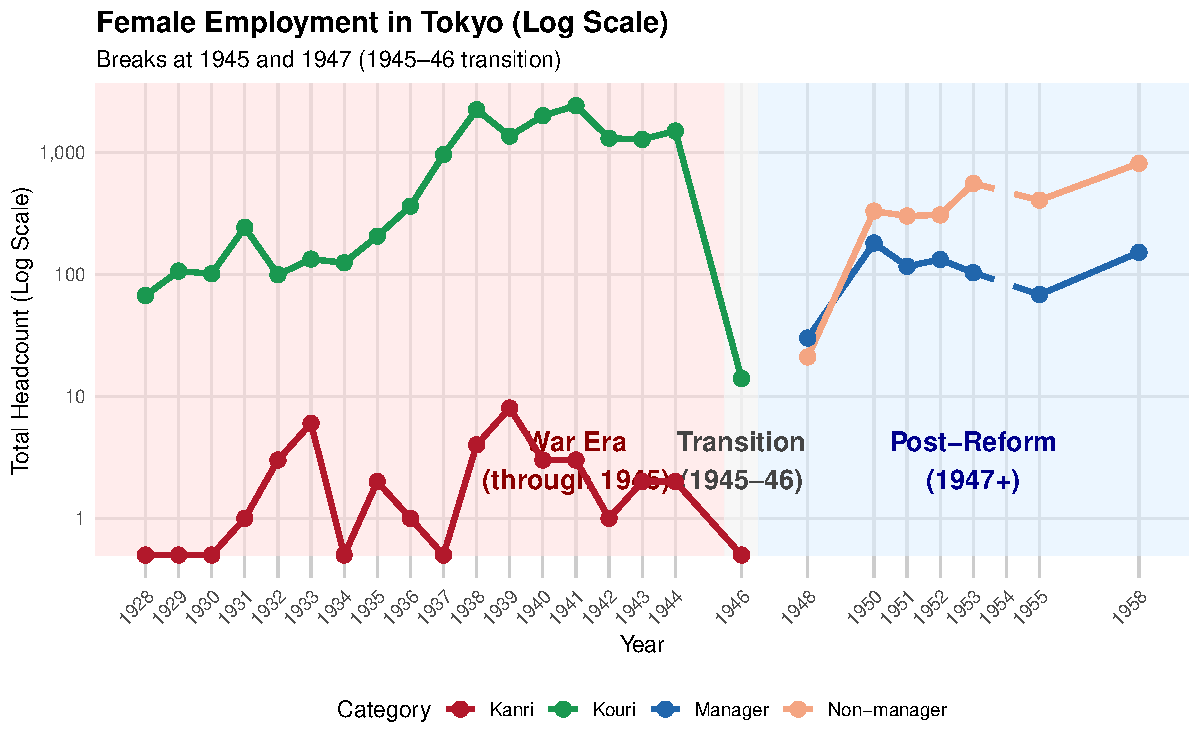
\includegraphics[width=0.9\linewidth]{Results/TimeSeriesChihouKomuin.pdf}
    \caption*{Note: Headcounts are shown on a log scale; the gap reflects the 1946-1949 transition period.}
    \label{fig:timeseries-chihoukomuin}
\end{figure}
\clearpage

\begin{figure}
    \centering
    \caption{Women in the Civil Service, 1928--1955}
    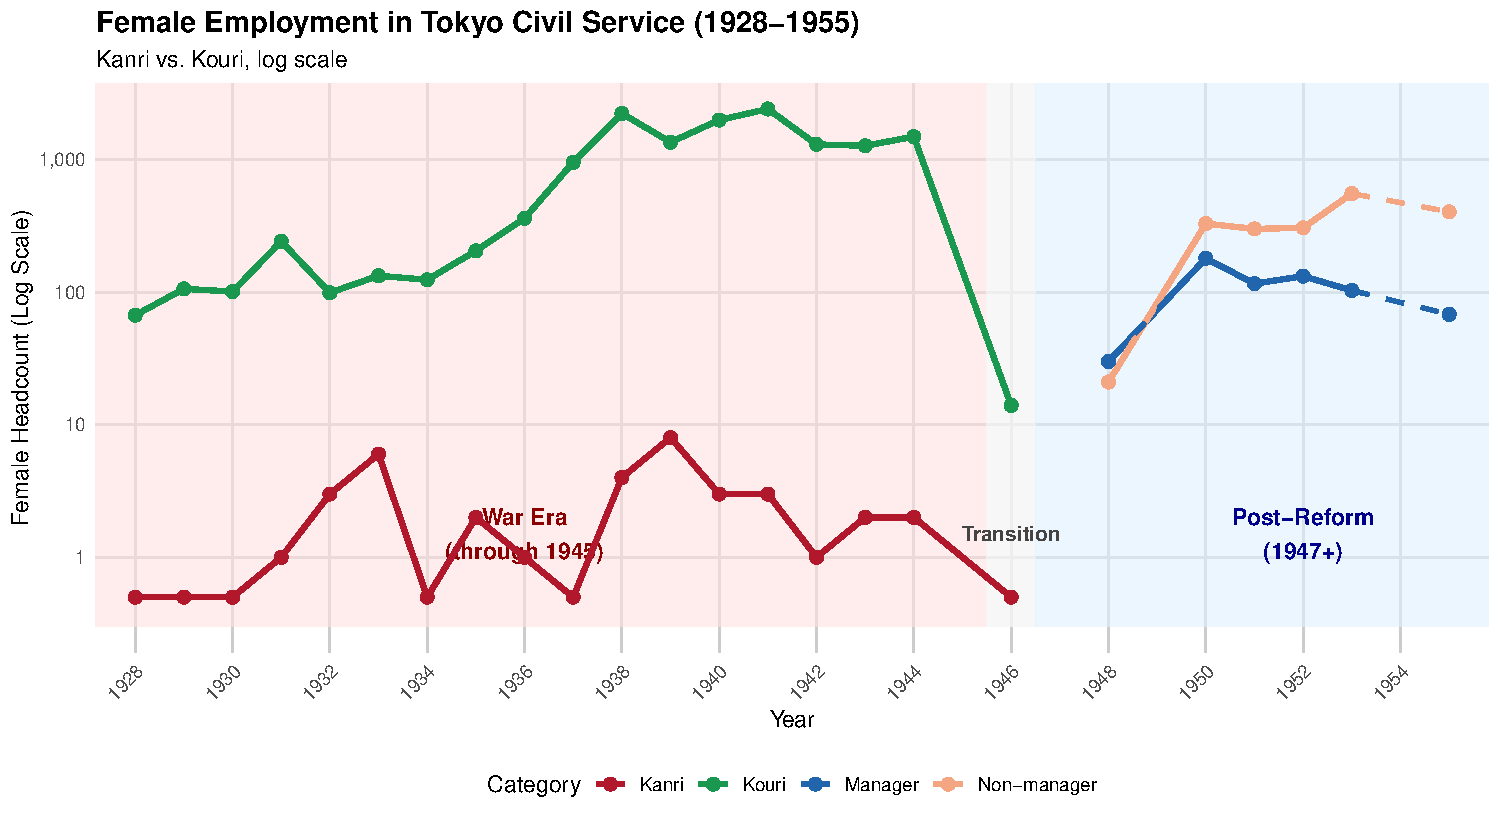
\includegraphics[width=0.9\linewidth]{Results/TimeSeriesWomen.pdf}
    \caption*{Note: Counts are shown on a log scale. Solid lines indicate observed data; dashed segments connect across gaps in the source records. \emph{Kanri} denotes appointed officials; \emph{Kouri} denotes public employees.}
    \label{fig:timeseries-women}
\end{figure}
